\chapter[Introduction]{Introduction}
\label{chap:intro}


%intorduccion del trabajo a realizar
%motivacion
%introducir proyecto en el que trabajas
%intruducir la empresa



Air pollution has emerged as one of the most pressing environmental challenges of the 21st century. Poor air quality has direct and well-documented impacts on human health, contributing to respiratory and cardiovascular diseases, and is linked to millions of premature deaths globally each year \cite{world2021global, nishida2022impact, rajagopalan2021pollution}. Among the most critical atmospheric pollutants are ozone (O$_3$), nitrogen dioxide (NO$_2$), and particulate matter (PM); these pollutants also have detrimental effects on ecosystems, reduce agricultural productivity, and play a significant role in climate change processes \cite{watson2016impact, fuzzi2015particulate, whoAmbientoutdoor}.

Nitrogen dioxide (NO$_2$) is a reactive gas primarily produced by high-temperature combustion in traffic, power generation, and industrial processes. Short-term exposure to NO$_2$ can irritate the respiratory tract and increase susceptibility to respiratory infections, particularly in vulnerable populations such as children and individuals with asthma. Long-term exposure is associated with the development of chronic respiratory diseases, including asthma, and with reduced lung function \cite{whoTypesPollutants, cao2025short, liu2021long}.

Ground-level ozone (O$_3$), in contrast to the protective ozone layer in the stratosphere, is a harmful secondary pollutant formed through photochemical reactions between nitrogen oxides (NO$_x$) and volatile organic compounds (VOCs) in the presence of sunlight. Due to its low solubility in water, ozone can penetrate deep into the lungs, inducing oxidative stress, airway inflammation, and reductions in lung function, particularly among sensitive groups such as individuals with asthma. Exposure to high concentrations of ground-level ozone has been associated with decreased lung function, exacerbation of asthma, increased hospital admissions, and a higher risk of respiratory morbidity, especially during summer smog events \cite{whoTypesPollutants, zheng2021short, tiotiu2020impact}.

Particulate matter (PM) is another key air pollutant, consisting of a complex mixture of solid and liquid particles suspended in the air. PM$_{10}$ refers to coarse particles smaller than 10 micrometers in diameter, which can reach the upper respiratory tract and cause irritation and respiratory symptoms. PM$_{2.5}$ refers to fine particles smaller than 2.5 micrometers; due to their small size, they can penetrate deep into the lungs and enter the bloodstream. PM$_{2.5}$ exposure has been strongly linked to cardiovascular disease, stroke, lung cancer, and premature mortality \cite{whoTypesPollutants, zarkeba2024relationship, xie2021toxicity, thangavel2022recent}. Because of these health risks, both PM$_{10}$ and PM$_{2.5}$ are widely used as key indicators in international air quality standards.

Beyond human health, these pollutants have severe environmental consequences. Elevated ozone concentrations damage crops and forests, reducing agricultural productivity and biodiversity. Nitrogen oxides and particulate matter contribute to soil acidification, water eutrophication, and climate forcing, disrupting natural ecosystems and accelerating global warming \cite{agathokleous2020ozone, europaQualityEurope}. As a result, monitoring and forecasting air quality have become essential tools for environmental policy, public health planning, and raising public awareness.

The urgency of this challenge is also recognized at the political and institutional level. Within the framework of the United Nations 2030 Agenda for Sustainable Development, several goals are directly related to the problem of air pollution. Goal 3 (Good Health and Well-Being) emphasizes the need to reduce illnesses caused by hazardous chemicals and air pollution; Goal 11 (Sustainable Cities and Communities) calls for improving urban air quality and reducing environmental impacts of cities; and Goal 13 (Climate Action) highlights the interconnections between air pollutants, greenhouse gases, and the fight against climate change. The European Union has also aligned its environmental policies with these objectives, reinforcing the importance of reliable air quality data for informed decision-making.


Here we have an image showing the referenced goals (Figure~\ref{fig:ej1}). 
A direct link can be found at the \href{https://sdgs.un.org/goals}{Sustainable Development Goals}.


\begin{figure}[h!btp]
	\centering
	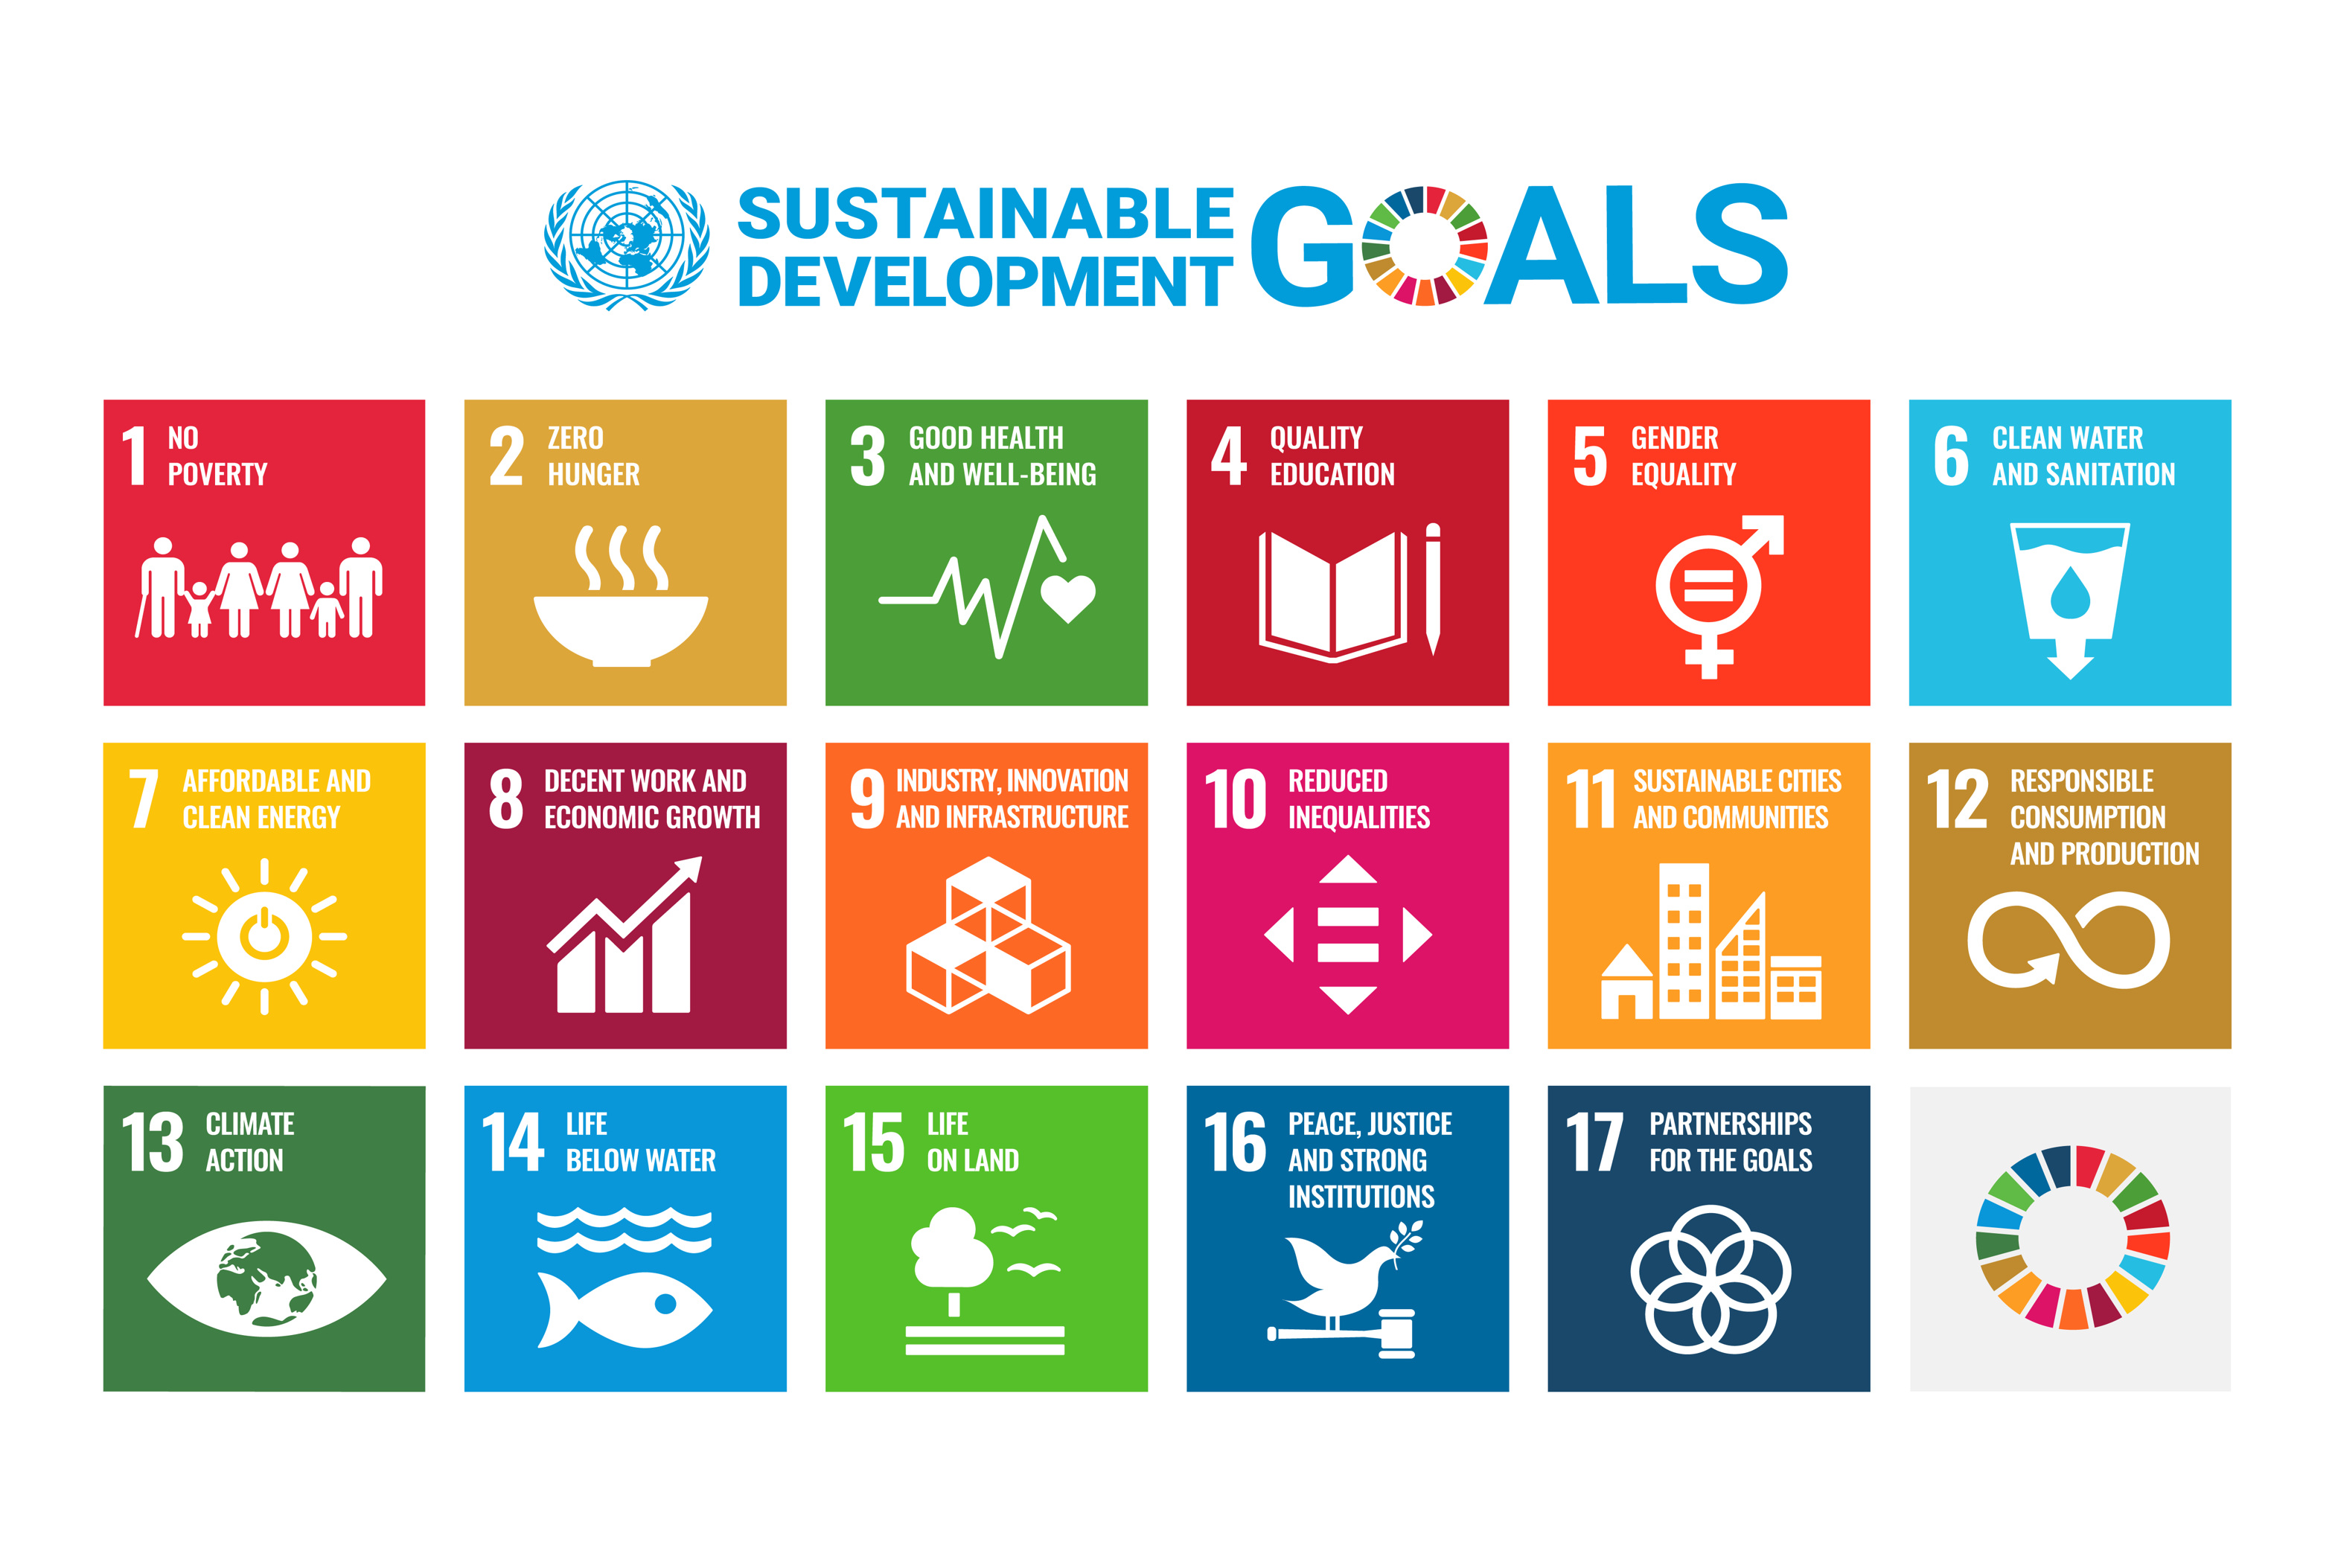
\includegraphics[width=0.7\textwidth]{fig/sustainable-image.png}
	\caption[Sustainable development goals]{Sustainable development goals.\footnotemark}
	\label{fig:ej1}
\end{figure}
\footnotetext{https://sdgs.un.org/goals}


\section{The Role of CAMS in Air Quality Forecasting}

To address the challenges posed by air pollution, advanced monitoring and forecasting systems are essential. One of them is the Copernicus Atmosphere Monitoring Service (CAMS), operated by the European Centre for Medium-Range Weather Forecasts (ECMWF), is one of the core components of the European Union's Earth observation programme Copernicus \cite{copernicusCopernicus,ecmwfECMWF}. You can think of CAMS as a weather forecast service for air pollution: instead of predicting rain or temperature, it predicts the state of the atmosphere and the levels of air pollutants. 

CAMS provides continuous, detailed information about the atmosphere, including daily forecasts for Europe and the whole world. It tracks a wide range of air pollutants, including those already introduced (PM${2.5}$, PM${10}$, O$_3$, NO$_2$, SO$_2$), and also several additional compounds.
Among them is carbon monoxide (CO), a colorless and odorless gas mainly emitted through incomplete combustion processes in vehicles, power generation, and industrial activities. At elevated levels, CO can impair the blood’s oxygen-carrying capacity, posing risks particularly for individuals with cardiovascular or respiratory conditions \cite{raub2000carbon}. CAMS also tracks ammonia (NH$_3$), a gas predominantly released by agricultural activities, including fertilizer application and livestock farming. In the atmosphere, ammonia contributes to the formation of secondary particulate matter, thus indirectly impacting both health and environmental quality \cite{wyer2022ammonia}.

Moreover, CAMS monitors methane (CH$_4$), a potent greenhouse gas that, while not directly toxic at ambient concentrations, plays a crucial role in long-term air quality and climate regulation by affecting atmospheric chemistry and radiative forcing \cite{lelieveld1993climate}. Similarly, carbon dioxide (CO$_2$), the principal anthropogenic greenhouse gas driving climate change, is included in CAMS observations due to its indirect effects on pollutant transport and weather patterns \cite{ebi2008climate}. Lastly, CAMS accounts for natural contributors to air quality such as dust, composed of fine soil particles lifted into the atmosphere by wind. These particles can significantly degrade air quality and cause respiratory irritation, especially in sensitive populations.

A key aspect of CAMS is its air quality forecasting system. In order to predict how pollution levels will evolve in different regions and over time, CAMS uses what are known as chemical transport models. These are sophisticated mathematical tools that simulate how pollutants behave and move through the atmosphere. Because weather conditions such as wind, temperature, and humidity affect how pollutants are dispersed, these models are closely coupled with meteorological forecasts.

To make these simulations as accurate as possible, CAMS incorporates real-world data from multiple sources. Satellite observations play a crucial role in capturing information about the atmosphere from space. These are complemented by in place measurements taken at ground level by air quality monitoring stations spread across different countries. By combining satellite data, surface observations, and advanced modeling, CAMS is able to produce near real-time analyses and forecasts.

The forecasting system works at both global and European scales. On a global level, CAMS provides forecasts with a spatial resolution of around 40 km, while in Europe, higher resolution models offer more detailed predictions down to scales of about 10 km.

This makes CAMS a key infrastructure for researchers, decision makers, and developers working on
climate and environmental services


Here we include the CAMS logo (Figure~\ref{fig:ej2}). A direct link to the service is available at the \href{https://atmosphere.copernicus.eu/}{CAMS webpage}.

\begin{figure} [h!btp]
	\centering
	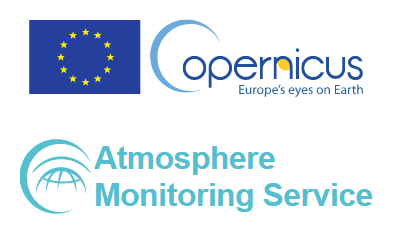
\includegraphics[width=0.7\textwidth]{fig/copernicus-image.png}
	\caption[CAMS]{Copernicus Atmosphere Monitoring Service (CAMS).\footnotemark}
	\label{fig:ej2}
\end{figure}
\footnotetext{https://atmosphere.copernicus.eu/}

   

\section{Motivation: Combining Visualization and Technical Analysis}

Although CAMS provides a large set of high-quality scientific data, accessing and using these data is not always straightforward for non-experts. Many of the available tools fall into two extremes. On the one hand, some platforms are designed mainly for researchers and specialists, offering the data in formats that require technical knowledge to be used. A common example is the so-called WMS (Web Map Service), which is a standardized way of delivering map images over the internet. In practice, a WMS layer is like a “raw map” containing pollutant concentrations, but it usually appears as a static image with little or no interactivity. Extracting numerical values or comparing pollutants across time and regions often requires additional software and expertise.

On the other hand, simplified applications focus only on highly aggregated indicators, such as the Air Quality Index (AQI). While these are easy to understand, they often hide important details, for example which specific pollutants are driving the problem, or how concentrations evolve during the day.

This project is motivated by the need to bridge this gap: to build a visualization tool that can take the detailed forecasts provided by CAMS and present them in a way that is both scientifically accurate and easy to explore. The idea is to allow users to interact with the data, select pollutants of interest, compare regions, and understand not only the overall air quality but also the underlying factors.

\section{Objectives of the Project}

The goal of this project is to make the advanced air quality forecasts provided by CAMS more accessible and understandable to a wider audience, while also gaining a deeper understanding of how these forecasts are produced and validated. To achieve this, the project pursues six main objectives that build on each other:

\begin{itemize}
	\item Understand CAMS forecasting models: Study how the system works, including the type of data it receives (from satellites, monitoring stations, and meteorological inputs) and how this information is processed to generate forecasts.
	\item Examine forecast evaluation methods: Analyze how the quality of CAMS predictions is checked against real-world measurements, identifying strengths and limitations of the current system.
	\item Explore WMS data access and pollutants representation: Investigate how Web Map Services (WMS) are used to deliver CAMS forecast layers, how pollutants are encoded and visualized, and what challenges arise when transforming these “raw map” layers into interactive formats.
	\item Develop a visualization platform: Create a web-based tool that transforms CAMS forecasts into interactive and user-friendly visualizations, enabling users to explore pollutant levels, compare regions, and better understand the factors driving air quality changes.
	\item Select relevant forecast variables: Review the full range of atmospheric variables predicted by CAMS, understand their meaning and relevance, and make a reasoned selection of those to be included in the visualization platform.
	\item Assess tools and implementation choices: Review the available software libraries and frameworks for working with CAMS data, compare their advantages and limitations, and document the reasoning behind the choices made for the visualization platform.  
	
\end{itemize}

Together, these objectives aim not only to enhance the scientific understanding of air quality forecasting, but also to provide a practical tool that bridges the gap between complex data and accessible information for decision-makers and the general public.
